\documentclass[12pt]{article}
%%% DOCUMENT FORMATTING %%%
\usepackage[margin=1in]{geometry}
\usepackage{enumitem}
\setlength{\parindent}{0pt}
\newcommand{\disp}{\displaystyle}

%%% HEADER %%%
\usepackage{fancyhdr}
\pagestyle{fancy}
\fancyhf{}
\lhead{MATH 1080}
\rhead{Vagnozzi}
\cfoot{\thepage}

%%% MATH NOTATION & SYMBOLS %%%
\usepackage{amssymb}
\usepackage{amsmath}
\newcommand{\R}{\mathbb{R}}
\newcommand{\N}{\mathbb{N}}
\newcommand{\Z}{\mathbb{Z}}
\newcommand{\lp}{\left(}
\newcommand{\rp}{\right)}
\newcommand{\ls}{\left[}
\newcommand{\rs}{\right]}
\newcommand{\lb}{\left\{}
\newcommand{\rb}{\right\}}
\newcommand{\arccot}{\text{arccot}}
\newcommand{\arccsc}{\text{arccsc}}
\newcommand{\arcsec}{\text{arcsec}} 

%%% TABLES %%%
\usepackage{colortbl}

%%% GRAPHS %%%
\usepackage{tikz}
\usepackage{pgfplots}
\pgfplotsset{compat=1.15}
\usepgfplotslibrary{fillbetween}
\usetikzlibrary{angles,quotes}

%%% ENVIRONMENTS %%%
\newcommand{\Example}{\paragraph{\Writinghand \hspace{0.1mm} Example.}}
\newcommand{\ExampleCont}{\paragraph{\Writinghand \hspace{0.1mm} Example (continued).}}
\newcommand{\boxenv}[2]{
	\fbox{
	\begin{minipage}{0.97\textwidth}
	\vspace{2mm}	
	\paragraph{#1} #2
	\vspace{2mm}
	\end{minipage}
	}}

%%% FUN THINGS %%%
\newcommand*\tc[1]{\tikz[baseline=(char.base)]{
            \node[shape=circle,draw,inner sep=2pt] (char) {#1};}}
\usepackage{marvosym}

%%% MISC %%%
\usepackage{hyperref}


\setcounter{page}{12}

\begin{document}
\section*{6.2: Regions Between Curves}

\boxenv{Learning Objectives.}{Upon successful completion of Section 6.2, you will be able to\dots
		
	\begin{itemize}[leftmargin=6mm]
		\item Answer conceptual questions about finding areas between curves.
		\item Find the area of a region using geometry.
		\item Find the area of a region (either by integrating with respect to $x$ or by integrating with respect to $y$) when the figure of the region is provided.
		\item Set up the area of a region in two ways: (1) in terms of one or more integrals with respect to $x$ and (2) in terms of one or more integrals with respect to $y$.
		\item Sketch a given region and find its area.
	\end{itemize}
	\vspace{-4mm}
}

\vspace{5mm}

\subsection*{Introduction}

In the next few sections, we will look at some geometric applications of integrals. In Calculus~I, we looked at the problem of finding the area between a curve $y=f(x)$ and the $x$-axis. Now, we are interested in finding the area between two or more curves.

\subsection*{Area Between Two Curves}

We want to find the area of a region bounded by the curves $y=f(x)$ and $y=g(x)$ on the interval $a\leq x \leq b$.

\vspace{60mm}

\boxenv{Definition.}{If $f$ and $g$ are continuous functions with $f(x)\geq g(x)$ on $[a,b]$, then the \textbf{area of the region} bounded by the curves $y=f(x)$, $y=g(x)$, and the lines $x=a$ and $x=b$ is

$$A=\int_a^b\big[ f(x)-g(x)\big]\,dx.$$}

\newpage

\Example Find the area enclosed by the curves $\textcolor{blue}{y=e^x}$, $\textcolor{red}{y=x^2-1}$, $x=-1$, and $x=1$.

\vspace{5mm}

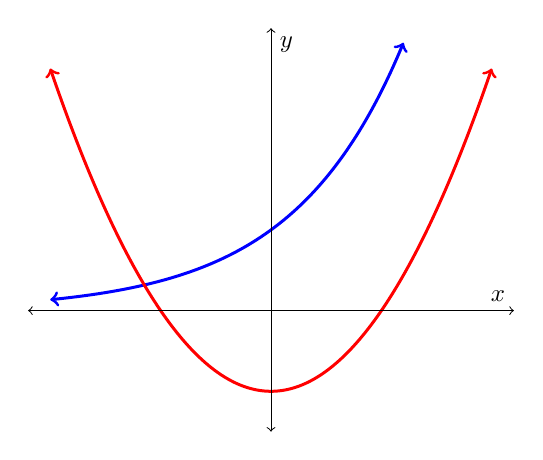
\begin{tikzpicture}[scale=.9]
	\begin{axis}[grid=none,
    	axis x line=middle,
    	xtick=\empty,
    	ytick=\empty,
        xmax=2.2, xmin=-2.2,
        axis y line=center,
        ymax=3.5, ymin=-1.5,
        axis line style=<->,
		xlabel=$x$,ylabel=$y$, 
		axis on top                    	
		]
    \addplot[<->,name path=f,smooth,domain=-2:1.2,color=blue,samples=100,very thick] {e^x};
    \addplot[<->,name path=g,smooth,domain=-2:2,color=red,samples=100,very thick] {x^2-1};
    \end{axis}
\end{tikzpicture}

\vspace{50mm}

\Example Find the area between $\textcolor{blue}{y=12-x^2}$ and $\textcolor{red}{y=x^2-6}$.

\vspace{5mm}

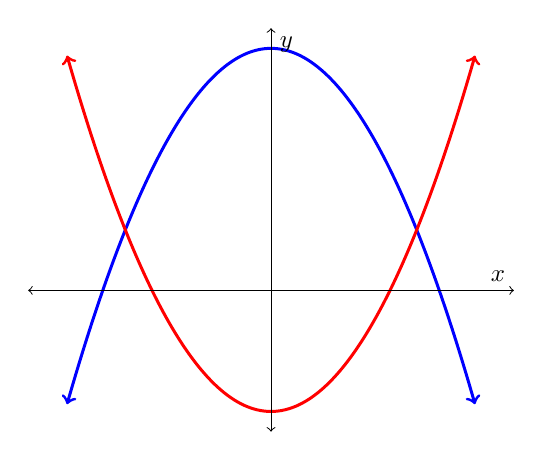
\begin{tikzpicture}[scale=.9]
	\begin{axis}[grid=none,
    	axis x line=middle,
    	xtick=\empty,
    	ytick=\empty,
        xmax=5, xmin=-5,
        axis y line=center,
        ymax=13, ymin=-7,
        axis line style=<->,
		xlabel=$x$,ylabel=$y$, axis on top                    	]
    \addplot[<->,name path=f,smooth,domain=-4.2:4.2,color=blue,samples=100,very thick] {12-x^2};
    \addplot[<->,name path=g,smooth,domain=-4.2:4.2,color=red,samples=100,very thick] {x^2-6};
    \end{axis}
\end{tikzpicture}

\newpage

\Example Find the area of the region enclosed by the curves $y=\cos x$, $y=\sin 2x$, $x=0$, and $x=\disp\frac{\pi}{2}$.

\vspace{5mm}

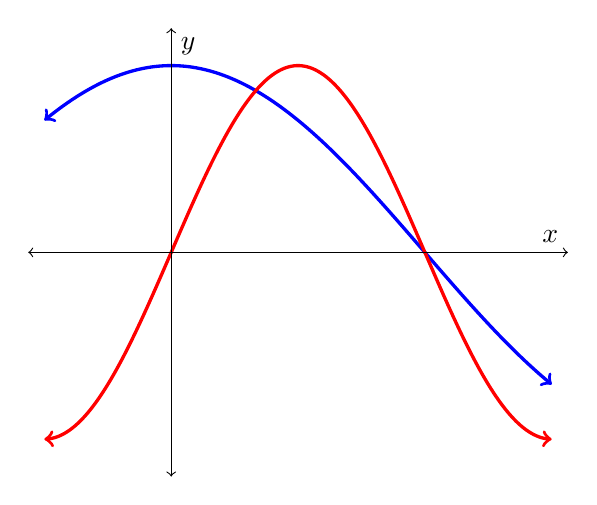
\begin{tikzpicture}
	\begin{axis}[grid=none,
    	axis x line=middle,
    	xtick=\empty,
    	ytick=\empty,
        xmax=3*pi/4+.1, xmin=-pi/4-.1,
        axis y line=center,
        ymax=1.2, ymin=-1.2,
        axis line style=<->,
		xlabel=$x$,ylabel=$y$, axis on top                    	]
    \addplot[<->,name path=f,smooth,domain=-pi/4:3*pi/4,color=blue,samples=100,very thick] {cos(deg(x))};
    \addplot[<->,name path=f,smooth,domain=-pi/4:3*pi/4,color=red,samples=100,very thick] {sin(deg(2*x))};
    \end{axis}
\end{tikzpicture}

\newpage

\Example Consider the region enclosed by $4x+y^2=12$ and $x=y$. Set up the integral(s) for the area\dots

\begin{enumerate}
\item[(a)] with respect to $x$. (You do not need to evaluate this integral.)

\vspace{5mm}

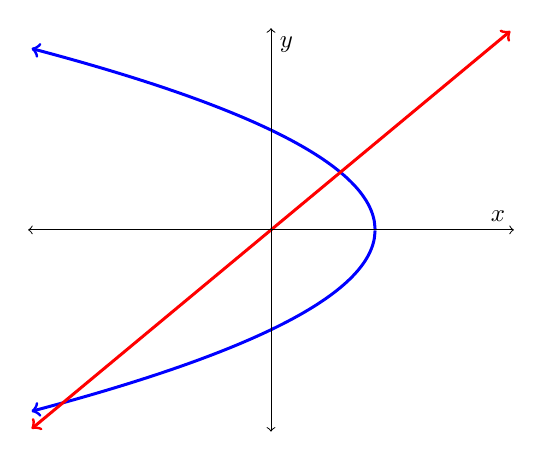
\begin{tikzpicture}[scale=.9]
	\begin{axis}[grid=none,
    	axis x line=middle,
    	xtick=\empty,
    	ytick=\empty,
        xmax=7, xmin=-7,
        axis y line=center,
        ymax=7, ymin=-7,
        axis line style=<->,
		xlabel=$x$,ylabel=$y$, axis on top                    	]
    \addplot[<-,name path=g,smooth,domain=-6.9:3,color=blue,samples=500,very thick] {sqrt(12-4*x)};
    \addplot[<-,name path=g,smooth,domain=-6.9:3,color=blue,samples=500,very thick] {-sqrt(12-4*x)};

    \addplot[<->,name path=g,smooth,domain=-6.9:6.9,color=red,samples=100,very thick] {x};
    \end{axis}
\end{tikzpicture}

\vspace{50mm}

\item[(b)] with respect to $y$. (Evaluate this one instead!)

\vspace{5mm}

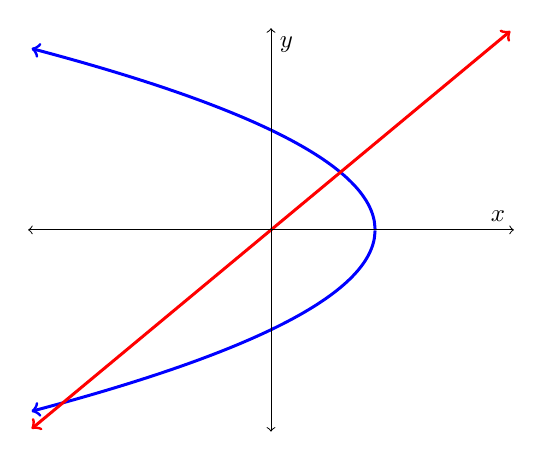
\begin{tikzpicture}[scale=.9]
	\begin{axis}[grid=none,
    	axis x line=middle,
    	xtick=\empty,
    	ytick=\empty,
        xmax=7, xmin=-7,
        axis y line=center,
        ymax=7, ymin=-7,
        axis line style=<->,
		xlabel=$x$,ylabel=$y$, axis on top                    	]
    \addplot[<-,name path=g,smooth,domain=-6.9:3,color=blue,samples=500,very thick] {sqrt(12-4*x)};
    \addplot[<-,name path=g,smooth,domain=-6.9:3,color=blue,samples=500,very thick] {-sqrt(12-4*x)};

    \addplot[<->,name path=g,smooth,domain=-6.9:6.9,color=red,samples=100,very thick] {x};
    \end{axis}
\end{tikzpicture}

\end{enumerate}
\end{document}